\documentclass{beamer}
\usepackage[utf8]{inputenc}

\usetheme{Madrid}
\usecolortheme{default}
\usepackage{amsmath,amssymb,amsfonts,amsthm}
\usepackage{txfonts}
\usepackage{tkz-euclide}
\usepackage{listings}
\usepackage{adjustbox}
\usepackage{array}
\usepackage{tabularx}
\usepackage{gvv}
\usepackage{lmodern}
\usepackage{circuitikz}
\usepackage{tikz}
\usepackage{graphicx}
\usepackage{mathtools}

\setbeamertemplate{page number in head/foot}[totalframenumber]

\usepackage{tcolorbox}
\tcbuselibrary{minted,breakable,xparse,skins}



\definecolor{bg}{gray}{0.95}
\DeclareTCBListing{mintedbox}{O{}m!O{}}{%
  breakable=true,
  listing engine=minted,
  listing only,
  minted language=#2,
  minted style=default,
  minted options={%
    linenos,
    gobble=0,
    breaklines=true,
    breakafter=,,
    fontsize=\small,
    numbersep=8pt,
    #1},
  boxsep=0pt,
  left skip=0pt,
  right skip=0pt,
  left=25pt,
  right=0pt,
  top=3pt,
  bottom=3pt,
  arc=5pt,
  leftrule=0pt,
  rightrule=0pt,
  bottomrule=2pt,
  toprule=2pt,
  colback=bg,
  colframe=orange!70,
  enhanced,
  overlay={%
    \begin{tcbclipinterior}
    \fill[orange!20!white] (frame.south west) rectangle ([xshift=20pt]frame.north west);
    \end{tcbclipinterior}},
  #3,
}
\lstset{
    language=C,
    basicstyle=\ttfamily\small,
    keywordstyle=\color{blue},
    stringstyle=\color{orange},
    commentstyle=\color{green!60!black},
    numbers=left,
    numberstyle=\tiny\color{gray},
    breaklines=true,
    showstringspaces=false,
}
\title{12.683}
\date{4th October, 2025}
\author{Puni Aditya - EE25BTECH11046}

\begin{document}

\frame{\titlepage}
\begin{frame}{Question}
The unit normal vector to the surface $X^2 + Y^2 + Z^2 - 48 = 0$ at the point (4, 4, 4) is \rule{2cm}{0.4pt}.
\end{frame}

\begin{frame}{Theoretical Solution}
Let the surface be defined by the level set of a function $f\brak{\vec{x}} = 0$.
\begin{align}
    f\brak{X, Y, Z} = X^2 + Y^2 + Z^2 - 48
\end{align}
The normal vector to the surface at any point is given by the gradient of the function, $\nabla f$.
\begin{align}
    \nabla f = \myvec{\frac{\partial f}{\partial X} \\ \frac{\partial f}{\partial Y} \\ \frac{\partial f}{\partial Z}} = \myvec{2X \\ 2Y \\ 2Z} \label{eq:27}
\end{align}
\end{frame}

\begin{frame}{Theoretical Solution}
Substituting 
\begin{align}
    \vec{p} = \myvec{4 \\ 4 \\ 4}
\end{align}
in \eqref{eq:27}
\begin{align}
    \vec{n} = \nabla f\brak{\vec{p}} = \myvec{2\brak{4} \\ 2\brak{4} \\ 2\brak{4}} = \myvec{8 \\ 8 \\ 8}
\end{align}
\end{frame}

\begin{frame}{Theoretical Solution}
To find the unit normal vector $\hat{\vec{n}}$,
\begin{align}
    \norm{\vec{n}} &= \sqrt{8^2 + 8^2 + 8^2} = \sqrt{3 \times 64} = 8\sqrt{3}
\end{align}
\begin{align}
    \hat{\vec{n}} = \frac{\vec{n}}{\norm{\vec{n}}} = \frac{1}{8\sqrt{3}}\myvec{8 \\ 8 \\ 8} = \frac{1}{\sqrt{3}}\myvec{1 \\ 1 \\ 1}
\end{align}
\end{frame}

\begin{frame}{Plot}
\begin{figure}[h!]
	\centering
	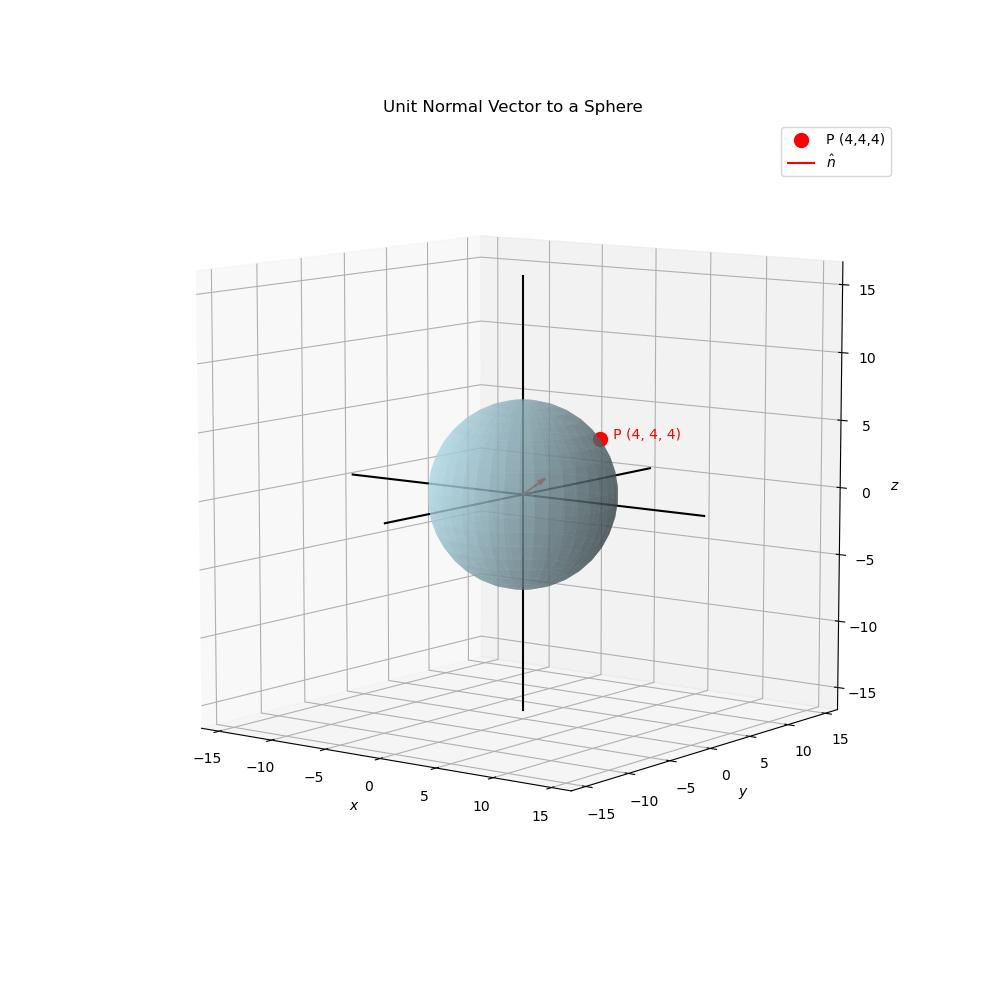
\includegraphics[width=0.5\columnwidth]{../figs/plot_c.jpg}
	\caption{Plot}
	\label{fig:fig}
\end{figure}
\end{frame}

\end{document}
